\documentclass{beamer}

\mode<presentation> {
\usetheme{AnnArbor}
}

\usepackage{graphicx}
\graphicspath{{./figures/}}
\usepackage{caption}
\usepackage{subcaption}
\usepackage{hyperref}
\hypersetup{colorlinks=true, citecolor=orange}
\usepackage{amsmath}
\usepackage{amsthm}
\usepackage{multirow}
\usepackage{natbib}
\usepackage{booktabs}
\usepackage{algorithm}
\usepackage{algpseudocode}

\setbeamertemplate{caption}[numbered]

\newtheorem{assumption}{Assumption}[section]
\newtheorem{proposition}{Proposition}
\newtheorem{remark}{Remark}[section]
\def\E{\mathbb{E}}
\def\P{\mathbb{P}}
\def\R{\mathbb{R}}
\def\ind{\perp\!\!\!\perp}
\DeclareMathOperator*{\argmin}{arg\,min}
\DeclareMathOperator*{\argmax}{arg\,max}

\title[Classification Diffusion Models]{Classification Diffusion Models: \\ Revitalizing Density Ratio Estimation}

\author{Victor Verma}
\institute[]
{
Department of Statistics \\
University of Michigan
}
\date[11/5/24]{11/5/24}

\begin{document}

\begin{frame}
    \titlepage
\end{frame}

\begin{frame}{Today's Paper}
    Today's paper: ``Classification Diffusion Models: Revitalizing Density Ratio Estimation''  by Yadin et al. (\cite{yadin2024clas}).

    \medskip

    It introduces Classification Diffusion Models (CDMs), which combine denoising diffusion models (DDMs) with density ratio estimation (DRE). The authors claim that
    \begin{itemize}
        \item Unlike DDMs, CDMs can provide the exact log-likelihood with a single neural function evaluation (NFE).
        \item CDMs denoises more accurately in terms of MSE than DDMs.
        \item CDMs, unlike other methods based on DRE, can successfully model some complex, high-dimensional distributions other than MNIST.
    \end{itemize}
\end{frame}

\begin{frame}{Computing Likelihoods for Generative Models}
    Being able to compute likelihoods for generative models $p(\mathbf{x})$ is useful. Two examples:
    \begin{itemize}
        \item Is a new sample $\mathbf{x^*}$ an outlier?
        \begin{itemize}
            \item Guess ``yes'' if $p(\mathbf{x^*})$ is low
        \end{itemize}
        \item Given two restorations $\mathbf{x^{(1)}}$ and $\mathbf{x^{(2)}}$ of an image, which is better?
        \begin{itemize}
            \item $\mathbf{x}^{(1)}$ if $p(\mathbf{x}^{(1)}) \ge p(\mathbf{x}^{(2)})$, otherwise $\mathbf{x}^{(2)}$
        \end{itemize}
    \end{itemize}
\end{frame}
    
\begin{frame}{Computing Likelihoods for DDMs: Two Approaches}
    \begin{enumerate}
        \item (Approximate) Estimate the likelihood by estimating the ELBO \cite{murphy2023prob}
        \[
        \E_q\left[\log p(x_T) + \sum_{t = 1}^T \log\frac{p_{\mathbf{\theta}}(\mathbf{x}_{t - 1} \mid \mathbf{x}_t)}{q(\mathbf{x}_t \mid \mathbf{x}_{t - 1})}\right]
        \]
        \begin{itemize}
            \item Requires many neural function evaluations (NFEs); recall that
            \begin{align*}            
                p_{\mathbf{\theta}}(\mathbf{x}_{t - 1} \mid \mathbf{x}_t) &= \mathcal{N}(\mathbf{x}_{t - 1} \mid \mathbf{\mu}_{\mathbf{\theta}}(\mathbf{x}_t, t), \mathbf{\Sigma}_{\mathbf{\theta}}(\mathbf{x}_t, t)), \\
                \mathbf{\mu}_{\mathbf{\theta}}(\mathbf{x}_t, t) &= \frac{1}{\sqrt{\alpha_t}}\left(\mathbf{x}_t - \frac{\beta_t}{\sqrt{1 - \overline{\alpha}_t}}\mathbf{\epsilon}_{\mathbf{\theta}}(\mathbf{x}_t, t)\right),
            \end{align*}
            where $\mathbf{\epsilon}_{\mathbf{\theta}}(\mathbf{x}_t, t)$ is a neural network
        \end{itemize}
        
        \item (Exact) Use an ODE solver as in \cite{song2021scor}
        \begin{itemize}
            \item \textbf{This isn't simple!}
        \end{itemize}
    \end{enumerate}
\end{frame}
    
\begin{frame}[allowframebreaks]{Exact Likelihood Computation for DDMs}
    Recall from Jingyang's presentation that the forward diffusion SDE is 
    \[
    d\mathbf{x} = \underbrace{-\frac{1}{2}\beta(t)\mathbf{x}}_{=: \mathbf{f}(\mathbf{x}, t)}\,dt + \underbrace{\sqrt{\beta(t)}}_{=: \mathbf{G}(\mathbf{x}, t)}\,d\mathbf{w}
    \]
    The corresponding probability flow ODE is \cite{song2021scor}:
    \[
    d\mathbf{x}
    = \left\{\mathbf{f}(\mathbf{x}, t) - \frac{1}{2}\nabla \cdot \left[\mathbf{G}(\mathbf{x}, t)\mathbf{G}(\mathbf{x}, t)^{\top}\right] - \frac{1}{2}\mathbf{G}(\mathbf{x}, t)\mathbf{G}(\mathbf{x}, t)^{\top}\nabla_{\mathbf{x}}\log p_t(\mathbf{x})\right\}\,dt
    \]
    Approximate the score $\nabla_{\mathbf{x}}\log p_t(\mathbf{x})$ by a neural network $\mathbf{s}_{\mathbf{\theta}}(\mathbf{x}, t)$:
    \[
    d\mathbf{x}
    = \underbrace{\left\{\mathbf{f}(\mathbf{x}, t) - \frac{1}{2}\nabla \cdot \left[\mathbf{G}(\mathbf{x}, t)\mathbf{G}(\mathbf{x}, t)^{\top}\right] - \frac{1}{2}\mathbf{G}(\mathbf{x}, t)\mathbf{G}(\mathbf{x}, t)^{\top}\mathbf{s}_{\mathbf{\theta}}(\mathbf{x}, t)\right\}}_{=: \mathbf{\tilde{f}}_{\mathbf{\theta}}(\mathbf{x}, t)}\,dt
    \]

    \framebreak

    Applying the instantaneous change of variables formula \cite{chen2018neur} yields:
    \begin{equation}\label{eq:chg_of_var_result}
        \log p_0(\mathbf{x}(0)) = \log p_T(\mathbf{x}(T)) + \int_{0}^{T} \nabla \cdot \mathbf{\tilde{f}}_{\mathbf{\theta}}(\mathbf{x}(t), t)\,dt
    \end{equation}

    $\nabla \cdot \mathbf{\tilde{f}}_{\mathbf{\theta}}(\mathbf{x}, t)$ can be expensive to compute; it can be estimated with the Skilling-Hutchinson trace estimator \cite{skilling1989thee, hutchinson1990stoc}:
    \[
    \nabla \cdot \mathbf{\tilde{f}}_{\mathbf{\theta}}(\mathbf{x}, t) = \mathbb{E}_{p(\mathbf{\epsilon})}[\mathbf{\epsilon}^{\top}\nabla\mathbf{\tilde{f}}_{\mathbf{\theta}}(\mathbf{x}, t)\mathbf{\epsilon}],
    \]
    where
    \begin{itemize}
        \item $\nabla\mathbf{\tilde{f}}_{\mathbf{\theta}}$ is the Jacobian of $\mathbf{\tilde{f}}_{\mathbf{\theta}}(\cdot, t)$
        \item $\mathbf{\epsilon}$ is a random variable such that $\mathbb{E}_{p(\mathbf{\epsilon})}[\mathbf{\epsilon}] = \mathbf{0}$, $\text{Cov}_{p(\mathbf{\epsilon})}[\mathbf{\epsilon}] = \mathbf{I}$
    \end{itemize}

    \framebreak

    Steps for computing the likelihood:
    \begin{itemize}
        \item Apply an ODE solver to the probability flow ODE to solve for $\mathbf{x}(t)$
        \item Sample from $p(\mathbf{\epsilon})$ to use the Skilling-Hutchinson trace estimator.
        \begin{itemize}
            \item Maybe do this for each $t$ and then numerically evaluate the integral in \eqref{eq:chg_of_var_result}?
        \end{itemize}
    \end{itemize}
    \textbf{This isn't simple!}

    \medskip

    The authors' idea: simplify likelihood computation using density ratio estimation.
\end{frame}

\begin{frame}[allowframebreaks]{Density Ratio Estimation}
    \textbf{Goal:} Estimate some unknown data density $p_d(\mathbf{x})$.
    
    \textbf{Idea:} For a known noise density $p_n(\mathbf{x})$, estimate $r(\mathbf{x}) := p_d(\mathbf{x}) / p_n(\mathbf{x})$, then estimate $p_d(\mathbf{x})$ as $\widehat{r(\mathbf{x})}p_n(\mathbf{x})$.

    \medskip

    Let
    \[
    z :=
    \begin{cases}
        1, & \mathbf{x} \sim p_d \\
        0, & \mathbf{x} \sim p_n
    \end{cases}
    \]
    so that
    \[
    r(\mathbf{x})
    = \frac{p_d(\mathbf{x})}{p_n(\mathbf{x})}
    = \frac{p(\mathbf{x} \mid z = 1)}{p(\mathbf{x} \mid z = 0)}.
    \]
    We have
    \[
    r(\mathbf{x})
    = \frac{p(z = 1 \mid \mathbf{x})p(\mathbf{x}) / p(z = 1)}{p(z = 0 \mid \mathbf{x})p(\mathbf{x}) / p(z = 0)}
    = \frac{p(z = 1 \mid \mathbf{x}) / p(z = 1)}{p(z = 0 \mid \mathbf{x}) / p(z = 0)}
    \]

    \framebreak

    We can estimate $r(\mathbf{x})$ by
    \[
    \widehat{r}(\mathbf{x}) :=
    \frac{\widehat{p}(z = 1 \mid \mathbf{x}) / \widehat{p}(z = 1)}{\widehat{p}(z = 0 \mid \mathbf{x}) / \widehat{p}(z = 0)}
    \]
    \textbf{Strategy:}
    \begin{itemize}
        \item Generate $\mathbf{x}^{(d, 1)}, \ldots, \mathbf{x}^{(d, M)} \sim p_d$, $\mathbf{x}^{(n, 1)}, \ldots, \mathbf{x}^{(n, N)} \sim p_n$
        \item Train a classifier $\widehat{p}(z = 1 \mid \mathbf{x})$ on $(\mathbf{x}^{(d, 1)}, 1), \ldots, (\mathbf{x}^{(d, M)}, 1), (\mathbf{x}^{(n, 1)}, 0), \ldots, (\mathbf{x}^{(n, M)}, 0)$
        \item Set $\widehat{p}(z = 1) = M / (M + N)$ and $\widehat{p}(z = 0) = N / (M + N)$
    \end{itemize}

    \smallskip
    
    This won't work well if $p_d$ and $p_n$ are very different (the \textbf{density chasm problem}).

    \framebreak

    Telescoping Density Ratio Estimation (TRE), introduced in \cite{rhodes2020tele}, provides a solution to the density chasm problem.

    \textbf{Goal:} Estimate $p_{\mathbf{x}_0}(\mathbf{x}) / p_{\mathbf{x}_m}(\mathbf{x})$, where $p_{\mathbf{x}_0}(\mathbf{x})$ is an unknown target density and $p_{\mathbf{x}_m}(\mathbf{x})$ is a known reference density.
    
    \textbf{Idea:} Write
    \[
    \frac{p_{\mathbf{x}_0}(\mathbf{x})}{p_{\mathbf{x}_m}(\mathbf{x})}
    = \frac{p_{\mathbf{x}_0}(\mathbf{x})}{p_{\mathbf{x}_1}(\mathbf{x})} \cdot \ldots \cdot \frac{p_{\mathbf{x}_{m - 1}}(\mathbf{x})}{p_{\mathbf{x}_m}(\mathbf{x})};
    \]
    $\mathbf{x}_i = \sqrt{\overline{\alpha}_i}\mathbf{x}_0 + \sqrt{1 - \overline{\alpha}_i}\mathbf{x}_m$ for $0 \le i \le m$ and $1 = \overline{\alpha}_0 \ge \ldots \ge \overline{\alpha}_m = 0$.

    \smallskip
    
    Then estimate $p_{\mathbf{x}_0}(\mathbf{x}) / p_{\mathbf{x}_m}(\mathbf{x})$ by estimating $p_{\mathbf{x}_i}(\mathbf{x}) / p_{\mathbf{x}_{i + 1}}(\mathbf{x})$ for each $i$ via binary classification.

    \framebreak

    TRE has two problems:
    \begin{itemize}
        \item $p_{\mathbf{x}_i}(\mathbf{x}) / p_{\mathbf{x}_{i + 1}}(\mathbf{x})$ is estimated only on $\mathbf{x} \sim p_{\mathbf{x}_i}$ and $\mathbf{x} \sim p_{\mathbf{x}_{i + 1}}$, so given $\mathbf{x}$, accuracy of $p_{\mathbf{x}_i}(\mathbf{x}) / p_{\mathbf{x}_{i + 1}}(\mathbf{x})$ estimate differs across $i$
        \item Accumulation of errors due to multiplying many ratios
    \end{itemize}

    TRE estimates well the distribution of MNIST, but not CIFAR-10:
    \begin{figure}
        \centering
        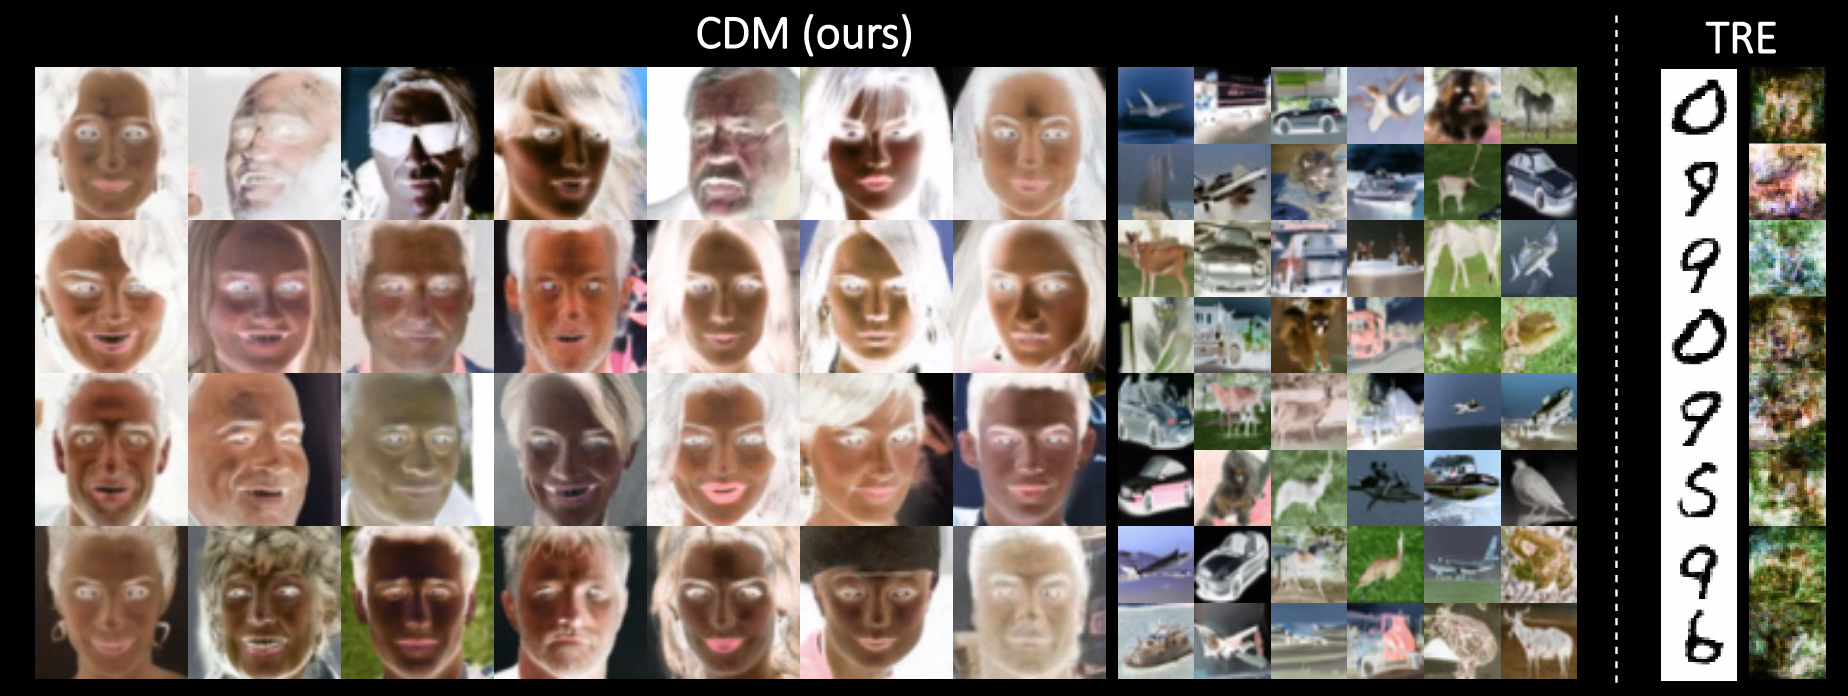
\includegraphics[width=0.78\linewidth]{cdm_fig1.png}
        \caption{Figure 1 in \cite{yadin2024clas}.}
        \label{fig:cdm_fig1}
    \end{figure}
\end{frame}

\begin{frame}[allowframebreaks]{Review of DDMs}
    \textbf{Forward Process:}

    \medskip

    $\mathbf{x}_0 \to \ldots \to \mathbf{x}_{T}$, where $\mathbf{x}_0$ represents an image, and
    \[
    \mathbf{x}_t = \sqrt{\alpha_t}\mathbf{x}_{t - 1} + \sqrt{1 - \alpha_t}\mathbf{\tilde{\epsilon}}_t, \quad \mathbf{\tilde{\epsilon}}_t \overset{\text{iid}}{\sim} \mathcal{N}(\mathbf{0}, \mathbf{I}).
    \]
    Alternatively, setting $\overline{\alpha}_t = \prod_{s = 1}^t \alpha_s$,
    \[
    \mathbf{x}_t = \sqrt{\overline{\alpha}_t}\mathbf{x}_0 + \sqrt{1 - \overline{\alpha}_t}\mathbf{\epsilon}_t, \quad \mathbf{\epsilon}_t \overset{\text{iid}}{\sim} \mathcal{N}(\mathbf{0}, \mathbf{I}).
    \]
    The $\alpha_t$'s are chosen from $(0, 1)$ so that $\overline{\alpha}_T \approx 0$ and $\mathbf{x}_T \sim \mathcal{N}(\mathbf{0}, \mathbf{I})$ roughly.

    \framebreak

    \textbf{Reverse Process:}

    \medskip

    Model $\mathbf{x}_{t - 1}$ given $\mathbf{x}_t$ as Gaussian such that
    \[
    \E[\mathbf{x}_{t - 1} \mid \mathbf{x}_t] = \frac{1}{\sqrt{\alpha_t}}\left(\mathbf{x}_t - \frac{1 - \alpha_t}{\sqrt{1 - \overline{\alpha}_t}}\epsilon_{\mathbf{\theta}}(\mathbf{x}_t, t)\right),
    \]
    $\epsilon_{\mathbf{\theta}}(\mathbf{x}_t, t)$ being a neural network, and $\text{Cov}[\mathbf{x}_{t - 1} \mid \mathbf{x}_t] = \sigma_t^2\mathbf{I}$.

    \medskip

    \textbf{Training:}

    \medskip

    We minimize the ELBO $\mathcal{L}(\mathbf{\theta}) := \sum_{t = 1}^T \E_{\mathbf{x}_0, \mathbf{\epsilon}_t}[\|\epsilon_{\mathbf{\theta}}(\mathbf{x}_t, t) - \mathbf{\epsilon}_t\|_2^2]$.

    \smallskip

    At convergence, $\epsilon_{\mathbf{\theta}}(x_t, t) \approx \E[\mathbf{\epsilon}_t \mid \mathbf{x}_t = x_t]$.
\end{frame}

\begin{frame}[allowframebreaks]{Denoising and Noise Level Classification}
    \textbf{Preliminaries:}

    \medskip

    \begin{itemize}
        \item Set $\overline{\alpha}_0 = 1$ and $\overline{\alpha}_{T + 1} = 1$.
        \item Let $p_{\mathbf{x}_t}$ be the density of $\mathbf{x}_t$.
        \item Let $\tilde{t}$ be a random variable supported on $\{0, \ldots, T + 1\}$ with pmf $p_{\tilde{t}}$.
        \item Let $\mathbf{\tilde{x}} = \mathbf{x}_{\tilde{t}}$ be the iterate at a random time $\tilde{t}$.
        \item We have
        \begin{itemize}
            \item $p_{\mathbf{x}_t}(x) = p_{\mathbf{\tilde{x}} \mid \tilde{t}}(x \mid t)$
            \item $p_{\mathbf{\tilde{x}}}(x) = \sum_{t = 0}^{T + 1} p_{\mathbf{x}_t}(x) p_{\tilde{t}}(t)$
        \end{itemize}
        \item The minimal cross-entropy classifier that predicts $\tilde{t}$ from $\mathbf{\tilde{x}}$ outputs
        \[
        (p_{\tilde{t} \mid \mathbf{\tilde{x}}}(0 \mid x), \ldots, p_{\tilde{t} \mid \mathbf{\tilde{x}}}(T + 1 \mid x)).
        \]
    \end{itemize}    

    \framebreak

    \begin{theorem}\label{thm:denoise_classify}
        Let $F(\mathbf{x}, t) = \log(p_{\tilde{t} \mid \mathbf{\tilde{x}}}(T + 1 \mid \mathbf{x})) - \log(p_{\tilde{t} \mid \mathbf{\tilde{x}}}(t \mid \mathbf{x}))$ with $\tilde{t}$, $\mathbf{\tilde{x}}$, and $\mathbf{x}_t$ as defined above.
        
        Then
        \[
        \E[\mathbf{\epsilon}_t \mid \mathbf{x}_t = x_t] = \sqrt{1 - \overline{\alpha}_t}(\nabla_{x_t}F(x_t, t) + x_t)
        \]
        regardless of the choice of the probability mass function $p_{\tilde{t}}$, provided that $p_{\tilde{t}}(t) > 0$ for all $t$.        
    \end{theorem}
\end{frame}

\begin{frame}{Exact Likelihood Calculation}
    \begin{theorem}
        For any $t \in \{0, 1, \ldots, T + 1\}$,
        \[
        p_{\mathbf{x}_t}(x) = \frac{p_{\tilde{t}}(T + 1)}{p_{\tilde{t}}(t)}\frac{p_{\tilde{t} \mid \mathbf{\tilde{x}}}(t \mid x)}{p_{\tilde{t} \mid \mathbf{\tilde{x}}}(T + 1 \mid x)}\mathcal{N}(x; \mathbf{0}, \mathbf{I}),
        \]
        where $\mathcal{N}(\cdot; \mathbf{0}, \mathbf{I})$ is the probability density function of a standard multivariate Gaussian distribution.
    \end{theorem}
    This is a simple consequence of one of the steps in the proof of Theorem~\ref{thm:denoise_classify}.
\end{frame}

\begin{frame}{Training for CDMs and DDMs}
    \begin{figure}[ht]
        \centering
        \begin{subfigure}[b]{0.45\textwidth}
            \centering
            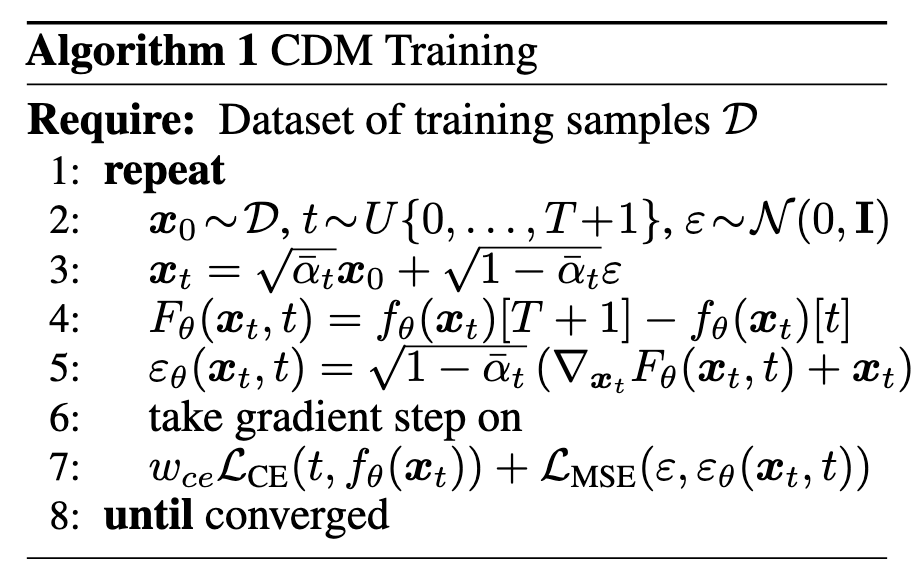
\includegraphics[width=\textwidth]{cdm_algo1.png}
            \caption{CDM Training \cite{yadin2024clas}}
            \label{fig:cdm_algo1}
        \end{subfigure}
        \hfill
        \begin{subfigure}[b]{0.55\textwidth}
            \centering
            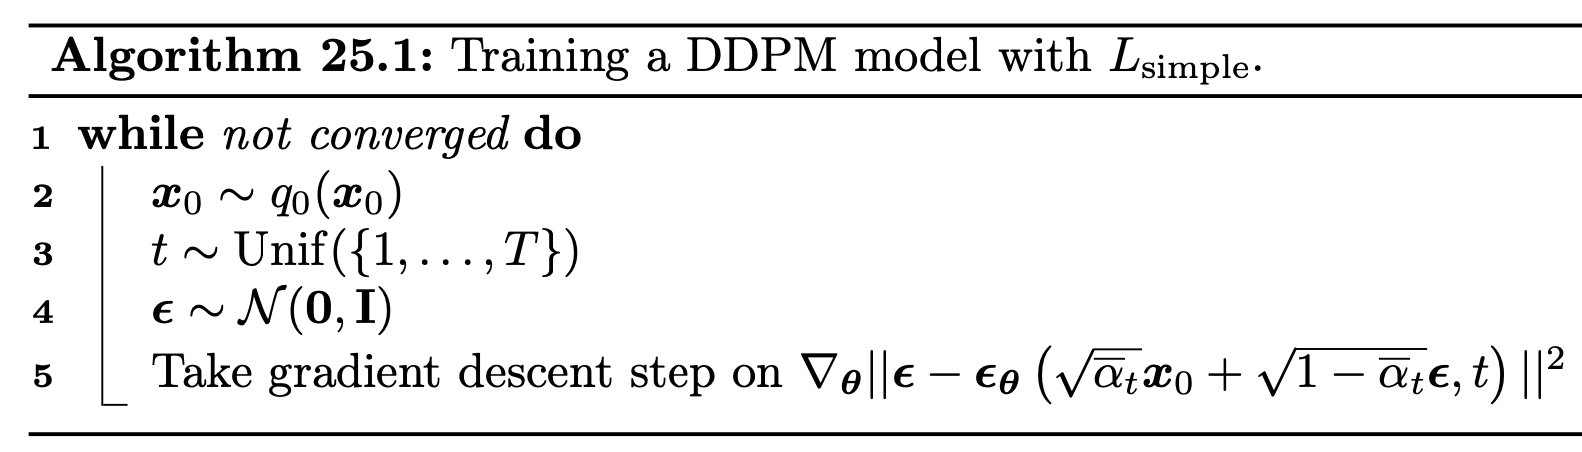
\includegraphics[width=\textwidth]{pml_algo25_1.png}
            \caption{DDPM Training \cite{murphy2023prob}}
            \label{fig:pml_algo25_1}
        \end{subfigure}
        \caption{Training for CDMs and DDPMs}
        \label{fig:training_algos}
    \end{figure}        
\end{frame}

\begin{frame}{Sampling for CDMs and DDMs}
    \begin{figure}[ht]
    \centering
    \begin{subfigure}[b]{0.45\textwidth}
        \centering
        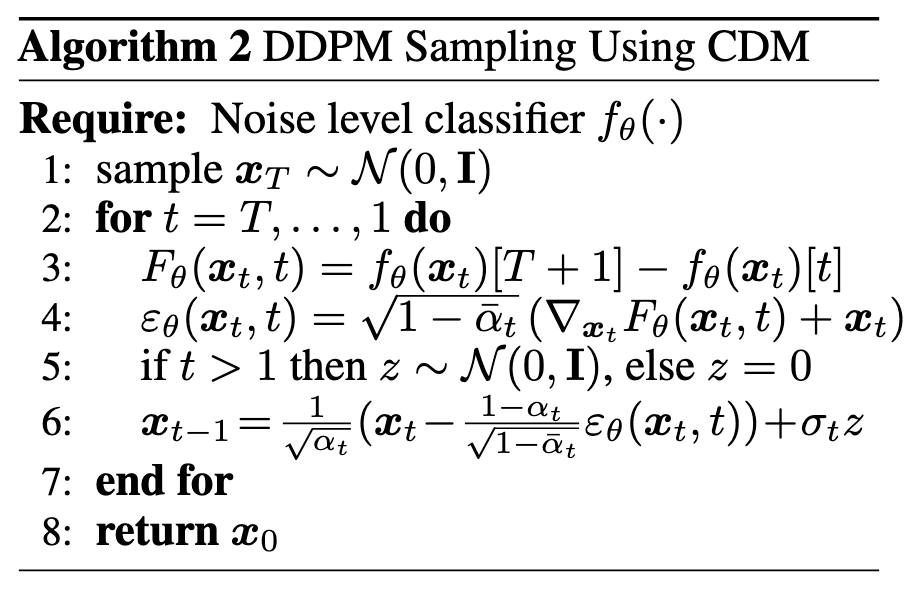
\includegraphics[width=\textwidth]{cdm_algo2.png}
        \caption{CDM Sampling \cite{yadin2024clas}}
        \label{fig:cdm_algo2}
    \end{subfigure}
    \hfill
    \begin{subfigure}[b]{0.45\textwidth}
        \centering
        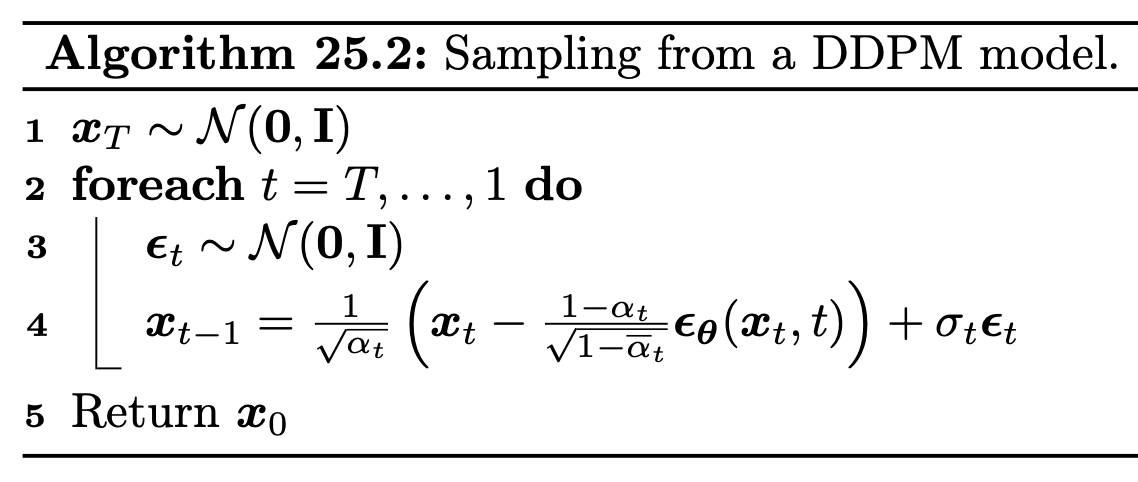
\includegraphics[width=\textwidth]{pml_algo25_2.png}
        \caption{DDPM Sampling \cite{murphy2023prob}}
        \label{fig:pml_algo25_2}
    \end{subfigure}
    \caption{Sampling for CDMs and DDPMs}
    \label{fig:algorithms}
\end{figure}
\end{frame}

\begin{frame}{The Fr\'{e}chet Inception Distance}
    \begin{itemize}
        \item The Fr\'{e}chet Inception Distance (FID) is used to evaluate the quality of images generated by generative models \cite{heusel2017gans}.
        \item It compares the distribution of generated images to the distribution of real images in a feature space.
        \item The Inception-v3 network (pre-trained on ImageNet) is used to extract features from both real and generated images into high-dimensional vectors.
        \item The FID is defined by
        \[
        \text{FID} := \sqrt{\|m_{\text{real}} - m_{\text{gen}}\|^2 + \text{Tr}(C_{\text{real}} + C_{\text{gen}} - 2(C_{\text{real}}C_{\text{gen}})^{1 / 2})}
        \]
        where $(m_{\text{real}}, C_{\text{real}})$ and $(m_{\text{gen}}, C_{\text{gen}})$ are the mean-covariance matrix pairs for the real and generated images, respectively.
    \end{itemize}
\end{frame}

\begin{frame}{Datasets}
    \begin{itemize}
        \item CIFAR-10 \cite{krizhevsky2009lear}: 60k images in 10 classes; 5:1 training:test ratio
        \item CelebA \cite{liu2015deep}: 200k+ images, 40 binary attributes per image
    \end{itemize}
    \begin{figure}[ht]
    \centering
    \begin{subfigure}[b]{0.45\textwidth}
        \centering
        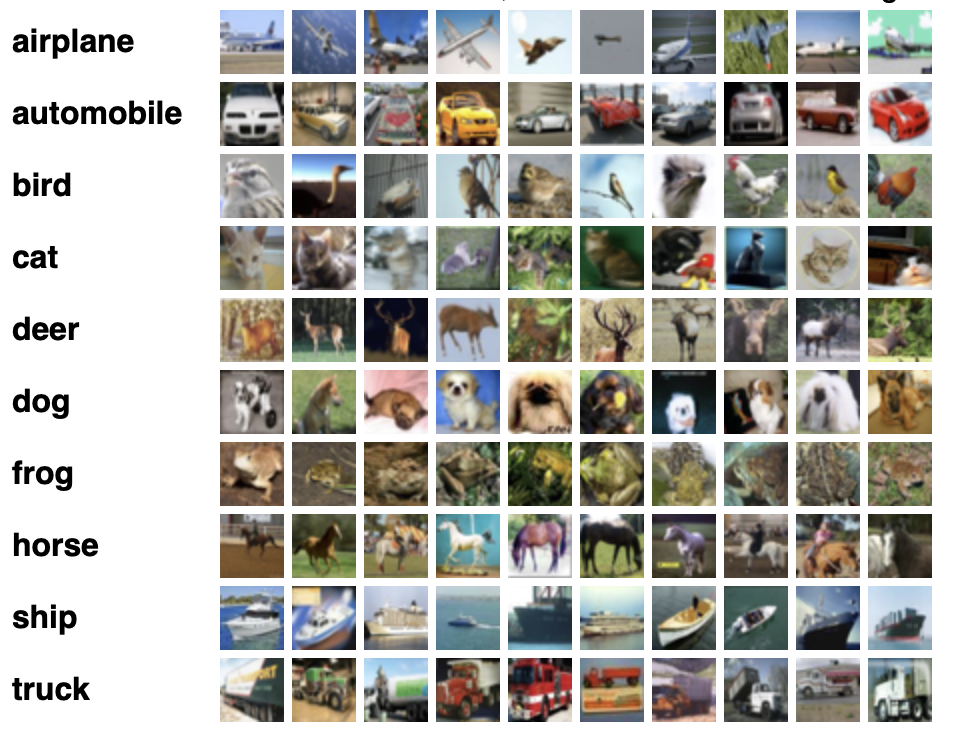
\includegraphics[width=\textwidth]{cifar-10.png}
        \caption{The CIFAR-10 classes \cite{krizhevsky2009lear}.}
        \label{fig:cifar-10}
    \end{subfigure}
    \hfill
    \begin{subfigure}[b]{0.45\textwidth}
        \centering
        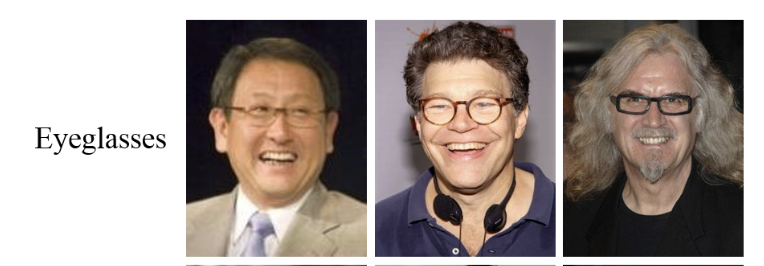
\includegraphics[width=\textwidth]{celeba.png}
        \caption{The CelebA dataset}
        \label{fig:celeba}
    \end{subfigure}
    \caption{}
    \label{fig:datasets}
\end{figure}
\end{frame}

\begin{frame}[allowframebreaks]{The Effects of Simplifying the Loss}
    \begin{itemize}
        \item CDMs were trained with the full loss, with the cross-entropy (CE) part omitted, and with the MSE part omitted.
        \item The CE, MSE, and negative log-likelihood (NLL) were evaluated on CIFAR-10; the FID was evaluated using 50k samples generated by a DDIM.
    \end{itemize}
    \begin{figure}
        \centering
        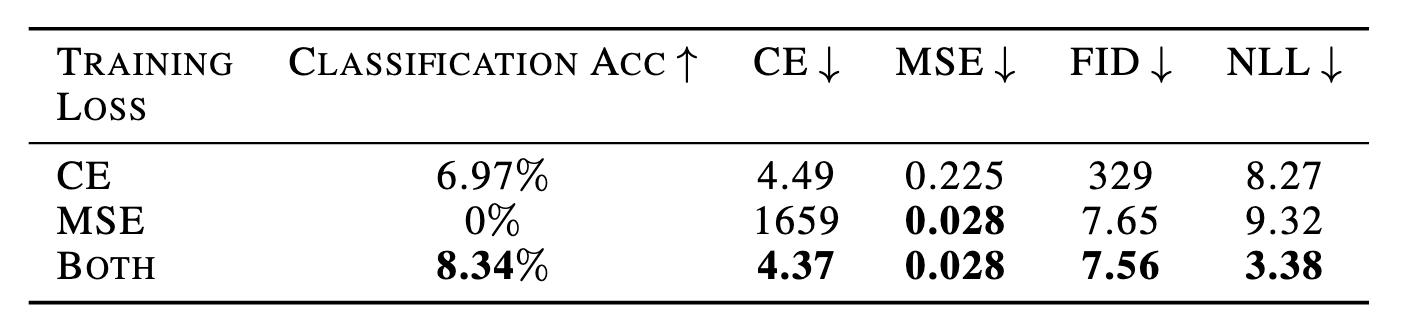
\includegraphics[width=0.75\linewidth]{cdm_tab1.png}
        \caption{Table 1 in \cite{yadin2024clas}}
        \label{fig:cdm_tab1}
    \end{figure}

    \framebreak

    The authors' explanation of why the CE part shouldn't be excluded:
    \begin{itemize}
        \item The MSE doesn't change if a function of $t$ is added to the model's output because it vanishes when taking the gradient with respect to x.
        \item The CE part removes the degree of freedom.
        \item Without the CE loss, the model can denoise but can't output the likelihood in one step.
    \end{itemize}

    \framebreak

    \begin{itemize}
        \item Another way to show that using both the CE and MSE parts is better than just using the CE part is to show the impact on $f_{\mathbf{\theta}}(x_t)$, which estimates $(\log p_{\tilde{t} \mid \mathbf{\tilde{x}}}(0 \mid x), \ldots, \log p_{\tilde{t} \mid \mathbf{\tilde{x}}}(0 \mid x))$.
        \item Using both parts yields better estimates (Figure~\ref{fig:cdm_fig3}).
        \begin{itemize}
            \item The estimate isn't only good at the correct value of $t$.
            \item The estimates decrease monotonically moving away from the correct value.
        \end{itemize}
    \end{itemize}

    \begin{figure}
        \centering
        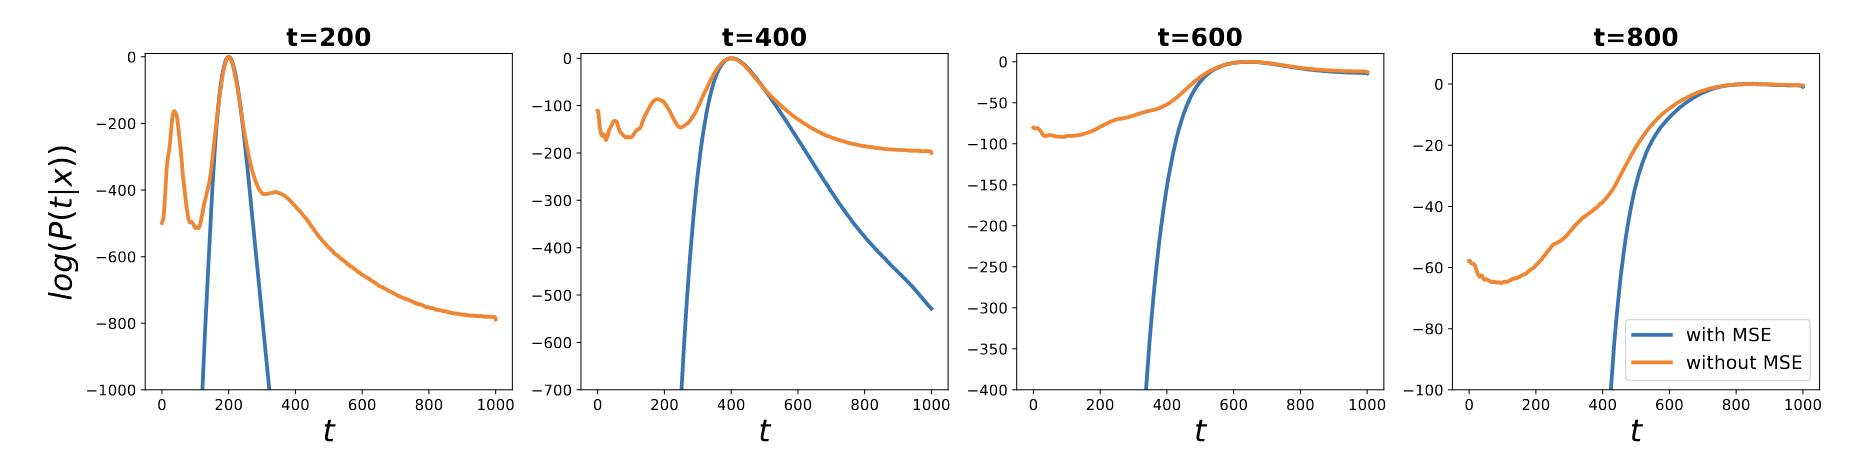
\includegraphics[width=0.75\linewidth]{cdm_fig3.png}
        \caption{Figure 3 in \cite{yadin2024clas}.}
        \label{fig:cdm_fig3}
    \end{figure}

    \framebreak

    The effects can also be evaluated based on sample images:
    \begin{figure}
        \centering
        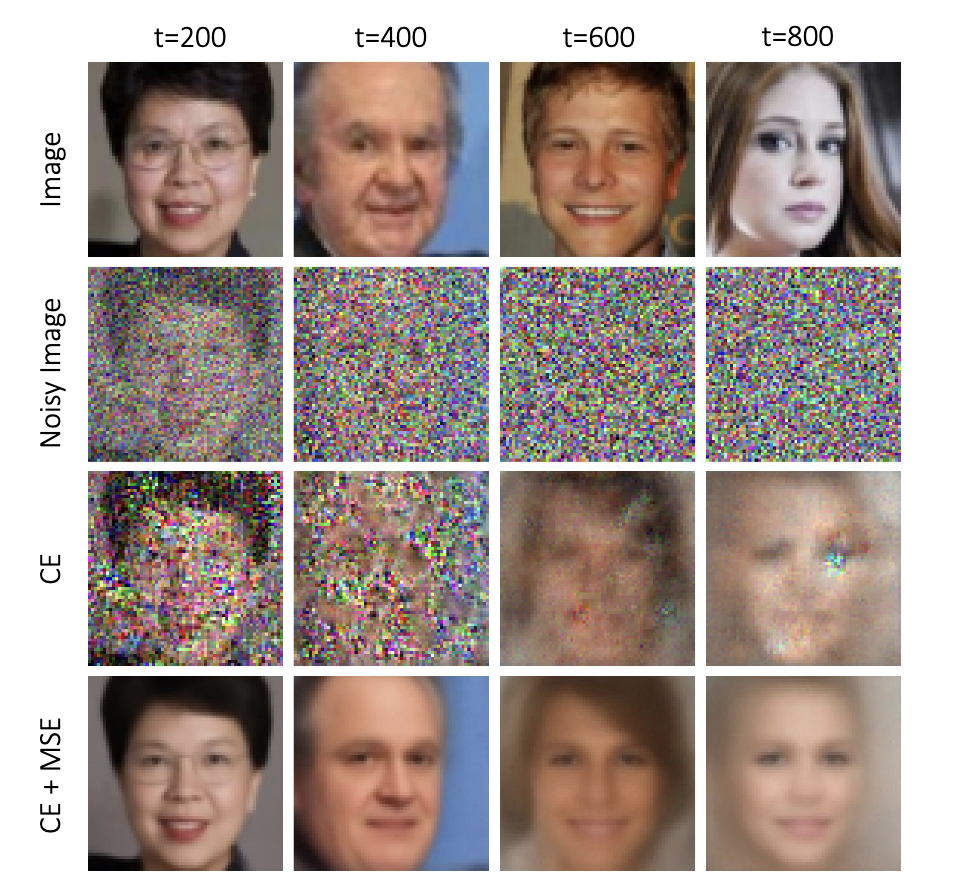
\includegraphics[width=0.5\linewidth]{cdm_fig8.png}
        \caption{Figure 8 in \cite{yadin2024clas}}
        \label{fig:cdm_fig8}
    \end{figure}
\end{frame}

\begin{frame}[allowframebreaks]{Denoising Performance}
    Denoising performance can be evaluated based on the MSEs:
    \begin{figure}
        \centering
        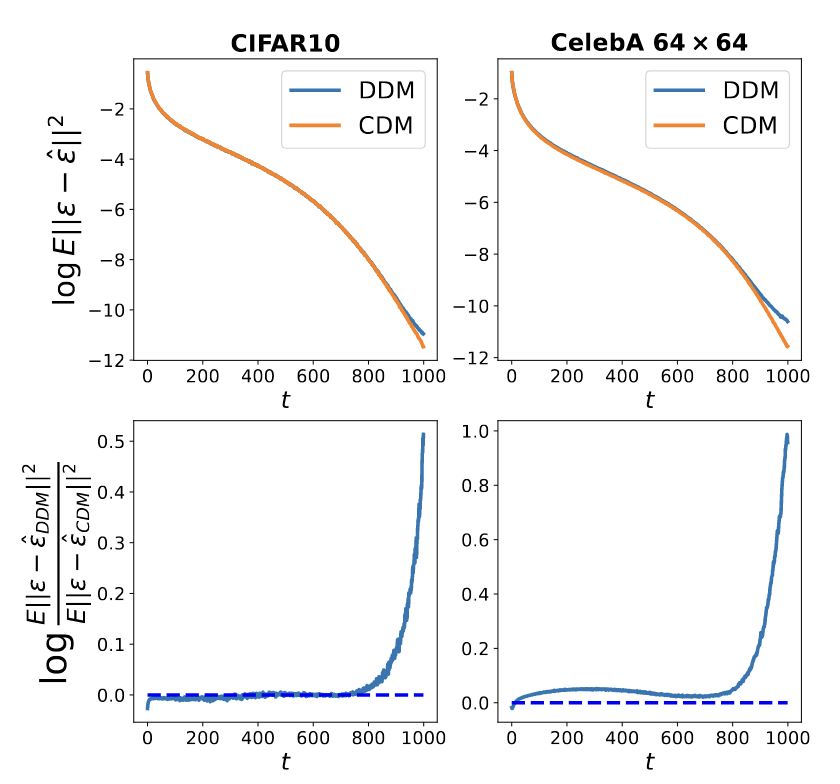
\includegraphics[width=0.48\linewidth]{cdm_fig4.png}
        \caption{Figure 4 in \cite{yadin2024clas}}
        \label{fig:cdm_fig4}
    \end{figure}

    \framebreak

    Denoising performance can also be evaluated based on sample images:
    \begin{figure}
        \centering
        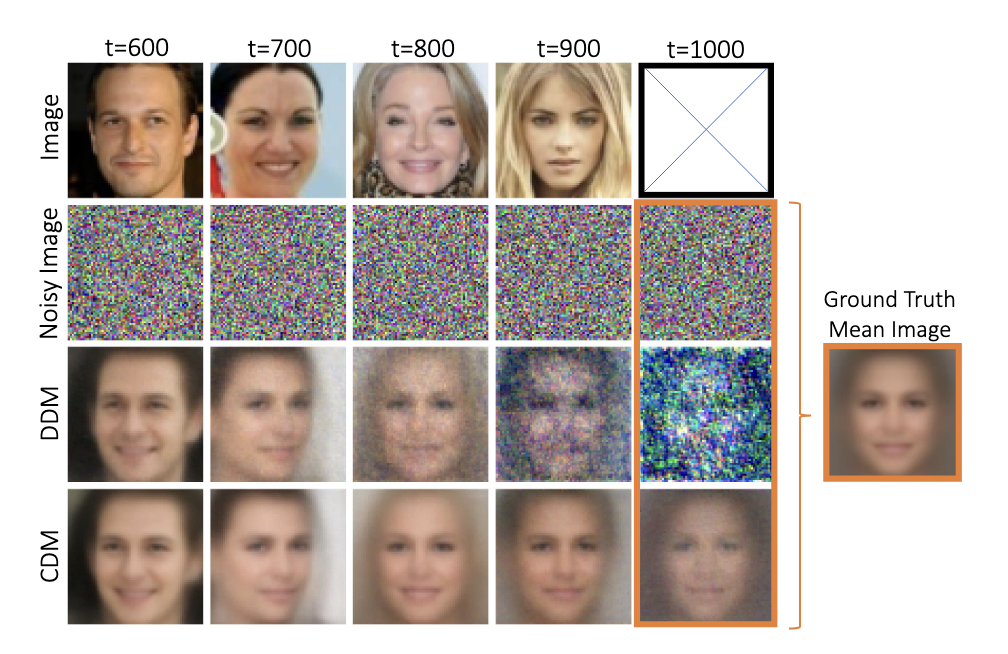
\includegraphics[width=0.5\linewidth]{cdm_fig5.png}
        \caption{Figure 5 in \cite{yadin2024clas}}
        \label{fig:cdm_fig5}
    \end{figure}
\end{frame}

\begin{frame}{Image Generation Quality}
    Image generation quality can be evaluated by computing FIDs:
    \begin{figure}
        \centering
        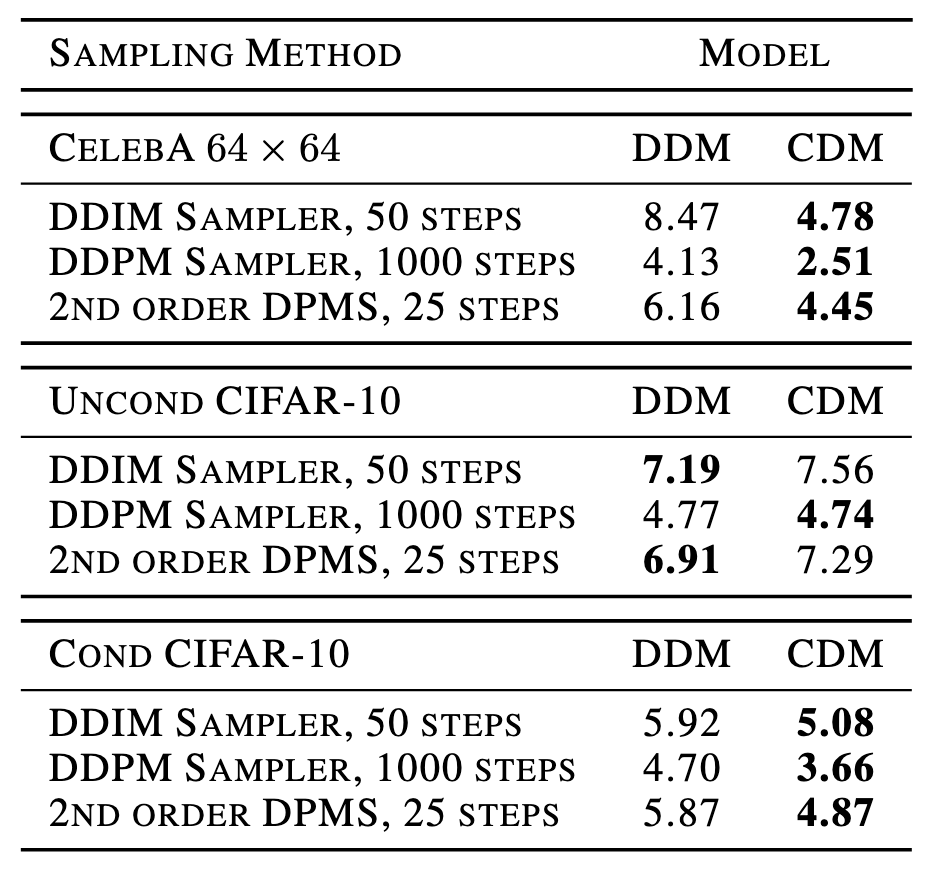
\includegraphics[width=0.5\linewidth]{cdm_tab2.png}
        \caption{Table 2 in \cite{yadin2024clas}}
        \label{fig:cdm_tab2}
    \end{figure}
\end{frame}

\begin{frame}{Negative Log-Likelihoods}
    CDMs are competitive in terms of negative log-likelihoods:
    \begin{figure}
        \centering
        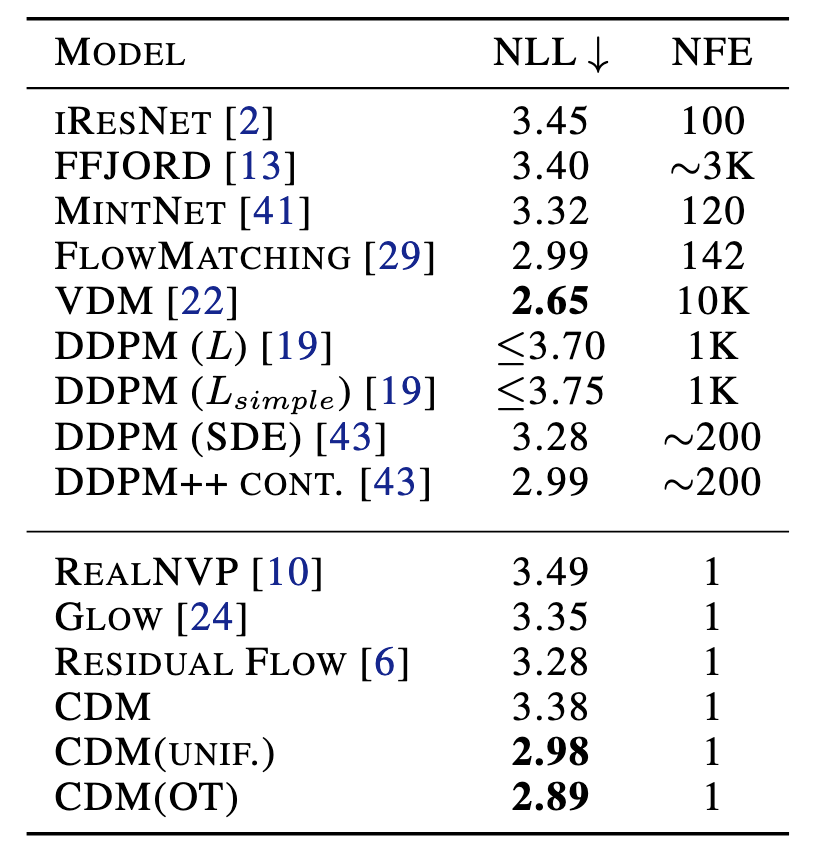
\includegraphics[width=0.5\linewidth]{cdm_tab3.png}
        \caption{Table 3 in \cite{yadin2024clas}}
        \label{fig:cdm_tab3}
    \end{figure}
\end{frame}

\begin{frame}[allowframebreaks]{References}
    \bibliographystyle{plain}
    \bibliography{bibliography}
\end{frame}

\end{document}